% !TEX root = ./proj_report.tex
\graphicspath{{mehul_pics/}}% Set graphics path location

\chapter{Introduction}
Removing noise from an original signal is a challenging problem receiving widespread attention from researchers. Digital images play an important role in experimental research and acquired images are often blurry and noisy and valuable information is concealed. Thus denoising and image sharpening becomes a necessary  preprocessing feature to retrieve an estimate of the underlying data  in analyzing images. This project aims to explore some of the widely used image enhancement algorithms to sharpen images and implement a robust metric to quantify the performance of filters under different blur sources in the image test cases where there is no reference clean image to compare with.\\

\noindent {\bf Experimental \& Analysis setup: }\\
The experimental and analysis setup for this project is as depicted in the following figure.
\begin{figure}[h!]
  \centering
                \centering
                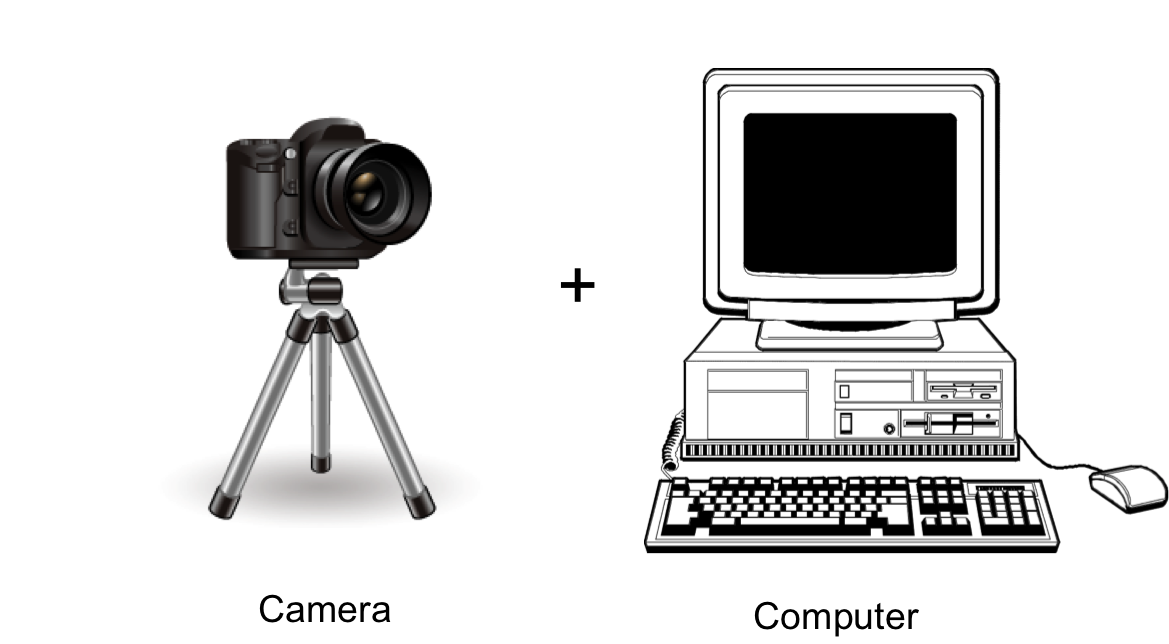
\includegraphics[width=.6\textwidth]{experimental_setup.png}
                \caption{Experimental setup consists of a good camera and a computer system. The camera captures images under pre-defined settings like focal length, shutter speed, aperture size and luminance while computer is used to perform image enhancement \& filter analysis.}
\end{figure}

\noindent Our analysis architecture is designed to meet the following objectives,
\begin{enumerate}
\item  Retrieve sharper image using different filter kernels. Training images are blurred using simulated standard point spread functions (PSF) and gaussian white noise of specified variance. Filter kernel characteristics are then compared against the true training image kernel to benchmark filter performance for the chosen degradation PSF and noise variance. 
\item Generally, the sharpness of an image is determined by human visual systems. This process can be automated and made simpler if there was a robust metric to evaluate the sharpness of a restored image and thus decide the optimum filter to restore a particular set of images. Three different sharpness metrics using different criteria have been implemented to automate the process of deblurring a no reference test image.
\end{enumerate}
\newpage